% !TeX root = ../Skript_HTML.tex
\cohead{\Large\textbf{Textauszeichnungen}}
\section{Textauszeichnungen}
Auf Webseiten können Teile von Texten ausgezeichnet werden, um sie hervorzuheben. Hierbei wird zwischen physischen und logischen Auszeichnungen unterschieden. Bei den physischen Auszeichnungen handelt es sich lediglich um optische Auszeichnungen, so dass Texte z.B. Fett oder Kursiv dargestellt werden. Eine besondere Bedeutung haben physisch ausgezeichnete Texte jedoch nicht. Bei logisch ausgezeichneten Texten, z.B. Überschriften oder Zitaten, ist das jedoch anders. Wenn man Texte logisch auszeichnet, dann erhalten die Texte auch eine entsprechende Bedeutung.

Ein Beispiel sind die beiden Tags \lstinline|<i>...</i>| und \lstinline|<em>...</em>|. Beide Tags stellen den Text in der Regel kursiv dar. Das \lstinline|<i>|-Tag steht für italic (deutsch kursiv). Es ist eine physische/optische Auszeichnung. Das \lstinline|<em>|-Tag steht für emphasize (deutsch hervorheben/betonen) und ist eine logische Auszeichnung, die in der Regel vom Browser ebenfalls als kursiver Text dargestellt wird. Wenn beide Tags zu kursivem Text führen, wo ist der Unterschied? Der Unterschied liegt im Wesentlichen darin, wie der Computer den Text auffasst:

Die beiden Sätze \lstinline|HTML ist <i>super</i> und toll| und \lstinline|HTML ist <em>super</em> und toll| werden im Browser zwar gleich angezeigt. Würde man jedoch eine KI fragen was HTML ist, so würde sie beim ersten Satz sagen, dass HTML super und toll ist und beim zweiten Satz, dass HTML insbesondere super ist und außerdem auch toll.

Seit HTML 5 sollen Texte auf Webseiten nur gemäß ihrer Bedeutung logisch ausgezeichnet werden. Das ist aus verschiedenen Gründen wichtig. Dazu zählen unter anderem:
\begin{itemize}
    \item Barrierefreiheit: Sehbehinderte bzw. blinde Menschen können die Texte auf Webseiten z.B. mit Screenreader lesen. Wenn Texte logisch ausgezeichnet werden, dann hilft das dabei, den Aufbau, die Struktur und die Inhalte der Webseite besser zu verstehen. Wenn man z.B. bei einem normalen Absatz lediglich die Schriftgröße so einstellt, dass es aussieht wie eine Überschrift, jedoch nicht als Überschrift auszeichnet, dann könnte man bei der Betrachtung am Bildschirm zwar annehmen, dass der Text eine Überschrift darstellen soll. Blinde Menschen können das jedoch nicht und für sie ist der Text ein ganz normaler Absatz. Daher ist es für sie eine große Hilfe, wenn man Texte gemäß ihrer Bestimmung auszeichnet.
    \item Auslesen durch Suchmaschinen: Die Aufnahme in die Suchmaschinen erfolgt in der Regel durch sogenannte Bots. Das sind Programme, die selbständig im Internet Webseiten auslesen und in den Suchmaschinenindex aufnehmen. Um die Struktur und die Inhalte einer Webseite zu erkennen und zu gewissen Suchbegriffen einzuordnen, wird unter anderem die Seite inkl. aller Texte und logischer Auszeichnungen ausgewertet. Kommt ein Begriff z.B. in einer Überschrift vor, so ist die Wahrscheinlichkeit, dass die Webseite interessante Infos zu diesem Begriff enthält größer, als wenn der Begriff nur im Fließtext vorkommt.
    \item Auslesen durch andere Programme: Was für Suchmaschinen gilt, das gilt auch für andere Programme wie z.B. LLMs/KIs, die Webseiten auslesen. Wenn z.B. in sozialen Netzwerken eine Webseite geteilt wird, wird häufig die Überschrift sowie ein Ausschnitt aus dem Text und evtl. ein Bild als Vorschau angezeigt. Wenn die Texte nicht entsprechend ausgezeichnet wurden (z.B. die Überschrift als Überschrift deklariert im Unterschied zu einfach die Schriftgröße vergrößert), dann werden solche Vorgänge erschwert.
    \item Aufbau einer Suchfunktion: Viele Webseiten nehmen nach einer gewissen Zeit sehr große Ausmaße an, sodass eine Suchfunktion auf der Webseite notwendig wird. Auch hierbei ist man darauf angewiesen, dass die Texte gemäß ihrer Bestimmung logisch ausgezeichnet werden. So kann man diesen eine gewisse Gewichtung verleihen. Wenn z.B. ein Suchbegriff auf verschiedenen Seiten in der Überschrift und in den Absätzen vorkommt, dann könnte man den Suchalgorithmus so programmieren, dass die Seite, die den Begriff in der Überschrift enthält eine höhere Gewichtung erhält. Man könnte die Suche auch so eingrenzen, sodass z.B. nur in den Überschriften gesucht wird.
\end{itemize}
\begin{Exercise}[title=Füge deiner Webseite Textauszeichnungen hinzu., label=Textauszeichnungen]

    Die Textelemente der Webseite sollen nun wie im Bild gezeigt ausgezeichnet werden. Zudem soll der spätere Betrachter wissen, um wessen Website es sich dabei handelt. Daher soll eine Überschrift eingefügt werden.
    \begin{minipage}[t]{\textwidth}
        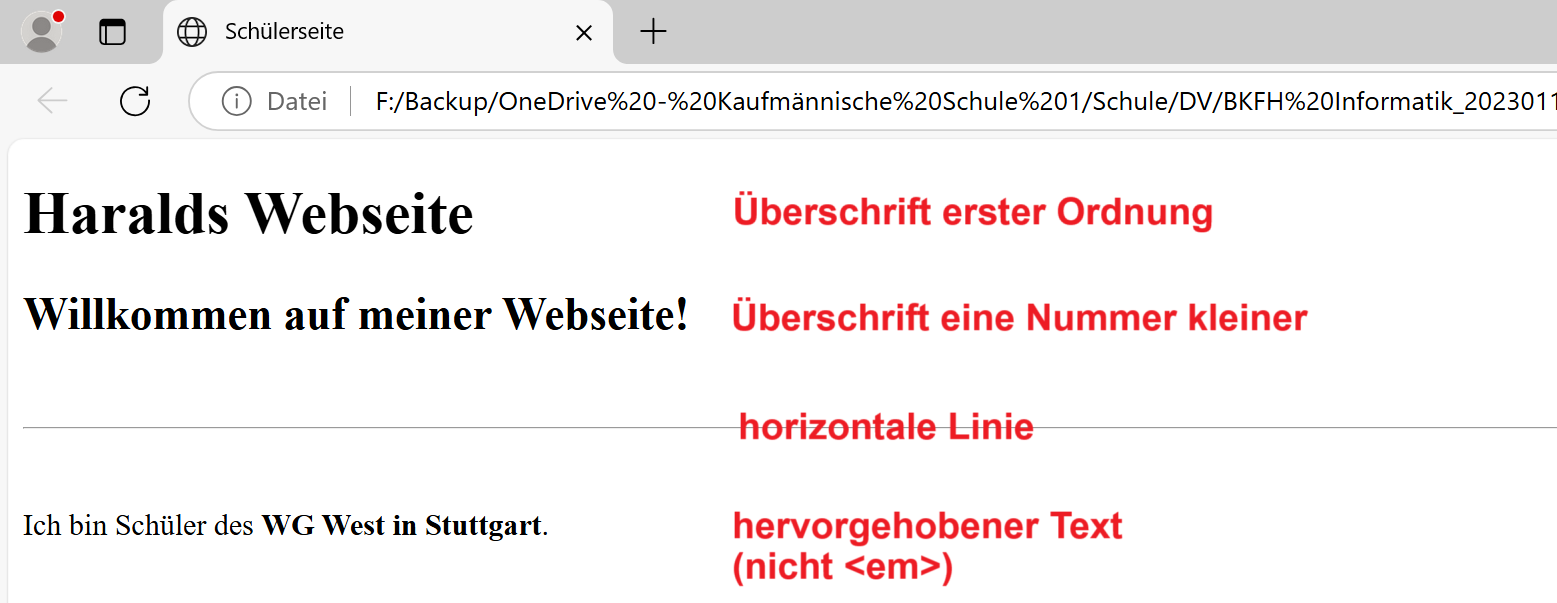
\includegraphics[width=\linewidth]{\pics/Textauszeichnungen.png}
    \end{minipage}
    Erweitere deine Datei \textit{schueler.html} mit dem Windows-Editor entsprechend der Vorgaben im Bild. Recherchiere dabei die notwendigen Tags.

    Validiere dann deine Datei \textit{schueler.html}.
\end{Exercise}


